\section{Defenses}
\label{sec:defenses}
% Budget: 1.25 pages. Source: DECISIONS.md s20, s21.5, s23, s24.1, s25.3, s25.5.
% - Policy-consistency blind spot: loss filtering recovers ~0% (s23).
% - D1 as pre-registered; missed its own sensitivity criterion (s20, s21.5).
% - Frontier vs kNN and no-skill baselines; uniform fails at ratio 0.9 (s24.1).
% - ShareCap: undominated in all 87 comparisons; cap curve (s25.3, s25.5).
% - Overhead: D1 ~781x cheaper than kNN; ShareCap near zero.
% - Counter-moves: padding (s21.6), volume (s21.4).
% Writing rule (docs/PAPER_PLAN.md): never say D1 is effective, or that ShareCap "beats"
% others (it is undominated, not shown superior in every comparison).
% TODO: prose.

\begin{figure}[t]
  \centering
  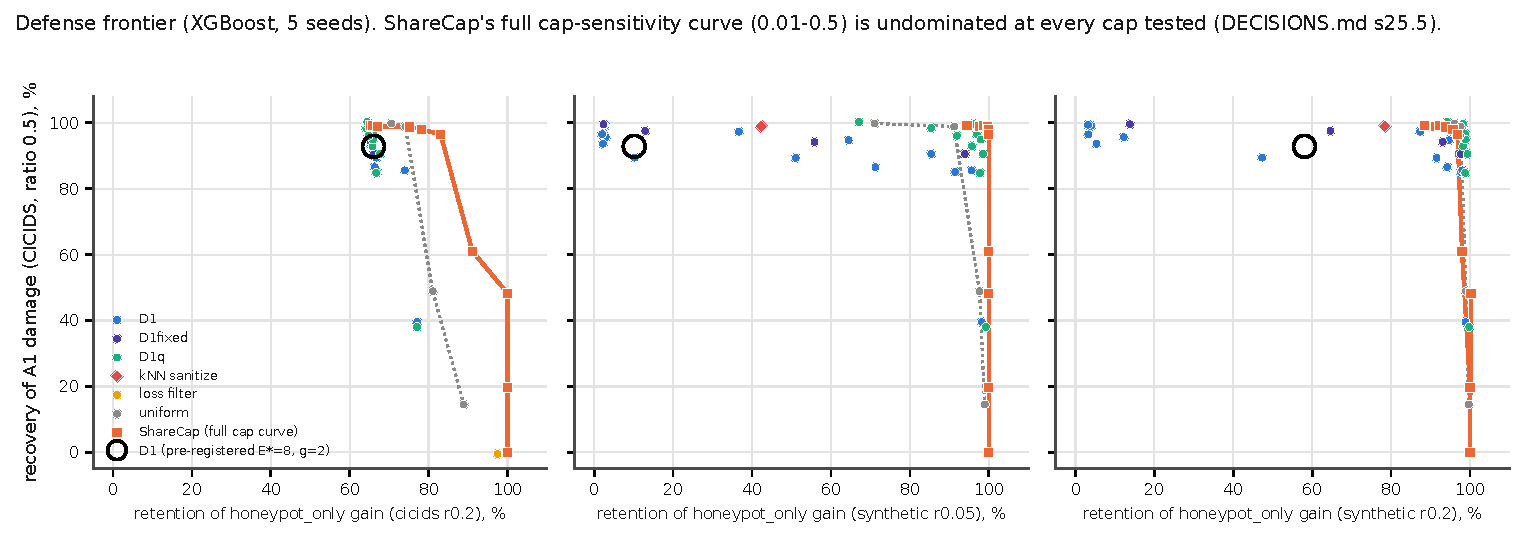
\includegraphics[width=\linewidth]{figures/F6_frontier.pdf}
  % Source: results/phase0/frontier/frontier_points.csv (D1/D1q/D1fixed/kNN/loss/uniform) +
  % results/phase0/loop/{cicids_recal,synthetic}/jobs/*sharecap_c*.csv (full ShareCap cap
  % curve, computed fresh in experiments/paper_figures.py:_sharecap_curve -- DECISIONS.md s25.5).
  % Regenerated by: python scripts/run.py figures --only F6
  \caption{TODO caption. Recovery of A1 damage (CICIDS, ratio 0.5) vs.\ retention of the
  honest loop's S0 gain, three retention axes. Points: D1 variants, kNN sanitize, loss
  filter, fixed-weight uniform down-weighting (dotted line: the no-skill baseline at each
  weight). Orange line: ShareCap's full cap-sensitivity curve, $c\in\{0.01,\ldots,0.5\}$.
  Circled: the pre-registered D1 configuration ($E^*=8,\gamma=2$).}
  \label{fig:f6-frontier}
\end{figure}

\begin{table}[t]
  \centering
  \caption{TODO: loss-filter recovery by ratio. Source: DECISIONS.md s23.}
  \label{tab:loss-filter}
  \begin{tabular}{lrr}
    \toprule
    Poison ratio & Recovery & Notes \\
    \midrule
    TODO & TODO & TODO \\
    \bottomrule
  \end{tabular}
\end{table}

\begin{table*}[t]
  \centering
  \caption{TODO: defense comparison. Source: DECISIONS.md s24.1, s25.3.}
  \label{tab:defense-comparison}
  \begin{tabular}{lrrrrr}
    \toprule
    Defense & Recovery r0.5 & Recovery r0.9 & Retention CICIDS & Retention synthetic & Overhead / round \\
    \midrule
    TODO & TODO & TODO & TODO & TODO & TODO \\
    \bottomrule
  \end{tabular}
\end{table*}
